\section{Limits of Non-Cooperative Delivery}\label{sec:limits}
Before designing cooperation we ask what any design without it can achieve.

\begin{definition}
A delivery scheme is \emph{non-cooperative} if every critical cell decodes only from packets that nodes of its own cell
received from the UAV. The trajectory, the speed profile, the code and the in-cell gathering are arbitrary.
\end{definition}
The class contains loitering with a rateless code \cite{zeng2018multicast}, both fountain-coded baselines of
Section~\ref{sec:eval}, and a hovering rotary-wing transmitter.

\subsection{A covering bound}
Let $F\subseteq\mathbb{R}^2$ be the set of horizontal positions the UAV may occupy and $P_k(x)$ the cell-level reception
probability \eqref{eq:pcell}. Consider the linear programme
\begin{equation}
\Lambda^\star=\max_{\lambda\ge0}\ \sum_{k\in K}\lambda_k\quad\text{s.t.}\quad \sum_{k\in K}\lambda_kP_k(x)\le1\ \ \forall x\in F.
\label{eq:lp}
\end{equation}
\begin{theorem}[Covering bound]\label{thm:cover}
Consider a non-cooperative scheme whose trajectory is fixed before take-off. If every critical cell is complete by time
$T$ with probability at least $1-\delta$, then
\begin{equation}
T\ \ge\ (1-\delta)\,Q\,\Tp\,\Lambda^\star .\label{eq:cover}
\end{equation}
\end{theorem}
\begin{IEEEproof}
Let $x_1,\dots,x_n$ be the emission positions up to time $T$, $n\le T/\Tp$, and $N_k$ the number of these packets heard
by at least one node of cell $k$. No code recovers $Q$ packets of information from fewer than $Q$ received packets, so
completion requires $N_k\ge Q$ and $\mathbb{E}[N_k]\ge Q\Pr\{N_k\ge Q\}\ge(1-\delta)Q$. By linearity of expectation
$\mathbb{E}[N_k]=\sum_{s=1}^nP_k(x_s)$. For any $\lambda$ feasible in \eqref{eq:lp},
\[
(1-\delta)Q\sum_k\lambda_k\le\sum_k\lambda_k\!\sum_{s=1}^n\!P_k(x_s)=\sum_{s=1}^n\sum_k\lambda_kP_k(x_s)\le n .
\]
Maximising over $\lambda$ gives $n\ge(1-\delta)Q\Lambda^\star$ and $T\ge n\Tp$.
\end{IEEEproof}

\begin{remark}[What $\Lambda^\star$ measures]
With $\bar p_k=\sup_{x\in F}P_k(x)$ we have $\max_k1/\bar p_k\le\Lambda^\star\le\sum_k1/\bar p_k$. If one position serves
every critical cell with probability one, $\Lambda^\star=1$: one airtime of the query suffices. If the reception
footprints are disjoint, $\Lambda^\star=\sum_k1/\bar p_k\ge|K|$: every critical cell needs its own airtime. In between,
$\Lambda^\star$ is the fractional number of critical cells that cannot be served simultaneously. By LP duality,
$\Lambda^\star$ is also the smallest total dwell, in units of $Q\Tp$, of a transmitter that could hover anywhere in $F$
and serve every cell in expectation; the bound is therefore tight, up to travel time and a concentration margin, for a
rotary-wing transmitter, and it can only be looser for a fixed-wing one.
\end{remark}
\begin{remark}[Robustness]
The proof uses only marginal reception probabilities. It holds for any dependence of fading across packets, for any code
and for any number of passes. Independence across the nodes of one cell enters only through the product form
\eqref{eq:pcell} of $P_k$.
\end{remark}

\subsection{Adding travel}
The covering bound ignores that the UAV must move between receivers. A second bound accounts for it when receivers are
far apart. For a radius $D$ let $p_k(D)=\sup\{P_k(x):\lVert x-c_k\rVert\ge D\}$, with $c_k$ the centre of cell $k$.
\begin{proposition}[Packing bound with travel]\label{prop:pack}
Let $S\subseteq K$ be critical cells whose centres are pairwise more than $2D$ apart, and let $W(S)$ be the weight of a
minimum spanning tree of $\{c_k\}_{k\in S}$ and the BS. Under the assumptions of Theorem~\ref{thm:cover},
\begin{equation}
\begin{aligned}
T\ \ge\ \min\Biggl\{&\frac{b\sum_{k\in S}\bar p_k^{-1}+(W(S)-2D|S|)^+/v_{\max}}{1+\sum_{k\in S}p_k(D)/\bar p_k},\\
&\frac{b}{\max_{k\in S}p_k(D)}\Biggr\},\qquad b=(1-\delta)Q\Tp .
\end{aligned}\label{eq:pack}
\end{equation}
\end{proposition}
The proof is in Appendix~\ref{app:pack}: emissions inside the disc of radius $D$ around $c_k$ serve $k$ with probability
at most $\bar p_k$, all others with at most $p_k(D)$; the discs are disjoint, and the path outside them connects them.
The second term of the minimum is the time before which no cell of $S$ can be served from outside its disc; it is not
binding in our evaluations.

\subsection{When cooperation is faster}
A single-pass scheme with ground cooperation must offer every cluster one copy of the query on its own cells, so its
flight lasts $T_{\mathrm{fly}}=\sum_c\max(\ell_c/v_c,\,Q\Tp)+T_{\mathrm{transit}}$, where $\ell_c$ is the path length
inside cluster $c$; the ground then needs a time $T_{\mathrm g}$ after the UAV has left.
\begin{corollary}[Sufficient condition]\label{cor:cross}
If a cooperative scheme completes every critical cell by
$T_{\mathrm{coop}}<(1-\delta)Q\Tp\Lambda^\star$, it completes before every non-cooperative scheme, whatever the latter's
trajectory and code.
\end{corollary}
Cooperation thus pays the query airtime $Q\Tp$ once per \emph{cluster}, while non-cooperation pays it once per unit of
$\Lambda^\star$. As the A2G range shrinks, $\Lambda^\star$ grows towards $|K|$ and beyond, whereas the number of clusters
is fixed by the network organisation.

\begin{corollary}[No-fly zones]\label{cor:nofly}
If $F$ excludes a region such that $\sup_{x\in F}P_k(x)=0$ for some critical cell $k$, then $\Lambda^\star=\infty$: no
non-cooperative scheme completes. A cooperative scheme is unaffected as long as the cell graph connects $k$ to cells
under the allowed path.
\end{corollary}

\subsection{Numerical evaluation}
We solve \eqref{eq:lp} on the three maps of Section~\ref{sec:eval} with the positions $x$ on a 50\,m grid and rescale
$\lambda$ by the maximum of $\sum_k\lambda_kP_k(x)$ on a 20\,m grid, so that the reported value is feasible on the finer
grid; \eqref{eq:pack} is maximised over $D$ and greedy choices of $S$. We take $\delta=0.1$ and $v_{\max}=50$\,m/s.
Table~\ref{tab:bounds} and Fig.~\ref{fig:bounds} compare the bounds with the measured schemes.

\begin{table}[t]\centering
\caption{Fractional covering number $\Lambda^\star$ and lower bounds on any non-cooperative scheme (s), against the
measured flight end of the fountain-coded baseline and of the single-pass flights (s). Maps with 8 / 12 / 15 clusters
and 45 / 66 / 92 critical cells.}\label{tab:bounds}
\setlength{\tabcolsep}{3pt}\footnotesize
\begin{tabular}{llrrrrrr}\toprule
Map & $R_{50}$ & $\Lambda^\star$ & \eqref{eq:cover} & \eqref{eq:pack} & FC+DTSP-N & \chord & \lmtour\\\midrule
8  & 1016 & 4.0  & 146  & 123  & 669  & 784  & 698\\
   & 498  & 10.0 & 362  & 256  & 1320 & 784  & 699\\
   & 199  & 23.2 & 842  & 610  & 2687 & 784  & 697\\
   & 99   & 35.3 & 1283 & 880  & 3305 & 784  & 708\\\midrule
12 & 1016 & 5.5  & 201  & 157  & 913  & 1292 & 1085\\
   & 498  & 14.1 & 511  & 339  & 2011 & 1292 & 1085\\
   & 199  & 33.5 & 1220 & 865  & 4016 & 1292 & 1083\\
   & 99   & 53.6 & 1951 & 1375 & 5078 & 1292 & 1082\\\midrule
15 & 1016 & 7.0  & 254  & 163  & 1134 & 1437 & 1394\\
   & 498  & 18.0 & 655  & 400  & 2563 & 1437 & 1308\\
   & 199  & 47.1 & 1713 & 1051 & 5567 & 1437 & 1293\\
   & 99   & 76.4 & 2779 & 1731 & 6808 & 1437 & 1291\\\bottomrule
\end{tabular}
\end{table}

\begin{figure*}[t]\centering
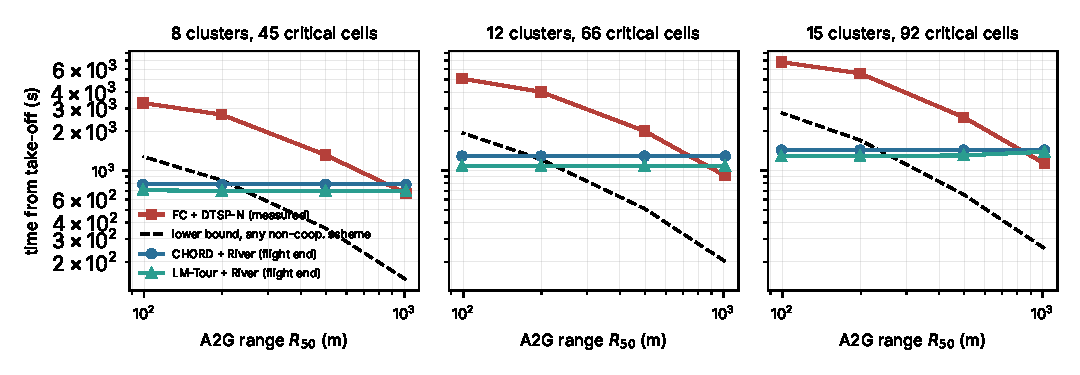
\includegraphics[width=0.86\textwidth]{bound-lp.pdf}
\caption{Lower bound on any non-cooperative scheme (maximum of \eqref{eq:cover} and \eqref{eq:pack}, dashed) against
the measured flight end of FC+DTSP-N and of the two single-pass flights, versus A2G range.}\label{fig:bounds}
\end{figure*}

Three observations follow. First, $\Lambda^\star$ grows by an order of magnitude from open land to $R_{50}=99$\,m, from
4--7 to 35--76, i.e., from below the number of clusters to several times it. Second, for $R_{50}\le200$\,m the covering
bound exceeds the time at which \lmtour{} has finished its \emph{entire} flight, return leg included, on all three maps
(e.g., 1713\,s against 1293\,s on the largest map at 199\,m), and at 99\,m it exceeds \chord's flight as well. On the
8-cluster map at 99\,m, where we have per-cell completion times, the last critical cell completes 746\,s after take-off
with \chord{}+River, against a bound of 1283\,s: no non-cooperative design, however it flies and codes, can match the
single pass there. Third, the bound is 2.4--4.6 times below the measured fountain-coded baseline. The gap has three
sources: the bound allows the transmitter to hover at the best position, it uses an ideal code without margin, and the
baseline's orbit and visiting order are heuristic. At $R_{50}\ge500$\,m the bound lies below the single-pass flight time
and certifies nothing, although the measured baseline is still slower from 500\,m downwards (Section~\ref{sec:eval}).

\emph{No-fly zone.} On the 8-cluster map we forbid the UAV to fly within a radius $\varrho$ of the centre of the cluster
with most critical cells. For $\varrho=400$\,m (two critical cells inside) the bound is unchanged. For $\varrho=700$\,m
(four inside) it stays at 145--363\,s for $R_{50}\ge498$\,m, jumps from 842 to 3431\,s at 199\,m, and is infinite at
99\,m: the cells deep inside cannot be reached from the air at all. \todo{ns-3 run of River with a path that avoids the
zone; not yet simulated.}
